\chapter{Series Management and Notes}
Notes are the most basic type of item known to Anathema. They consist of nothing more than a title and a formatted text 
field, allowing you to keep track of things fitting nowhere else or preparing simple texts for game sessions.
Basic text styles (bold, italics, underline) are selected either by clicking the respective button or via the established hotkeys (CTRL+B / I / U).

Series Management is more complex, but usage is fairly straightforward as well. To the left of the screen (cf. figure \ref{fig:Series}), the series plot tree is displayed. Use the right-click menu or the buttons provided to add Stories, Episodes and Scenes, afterwards select them to provide titles and descriptions in the editors to the right. Basic text styles are supported as well.

The tree supports reordering operations, either via the up/down controls on the bottom of the screen or by drag-and-dropping.

\begin{figure}
	\centering
		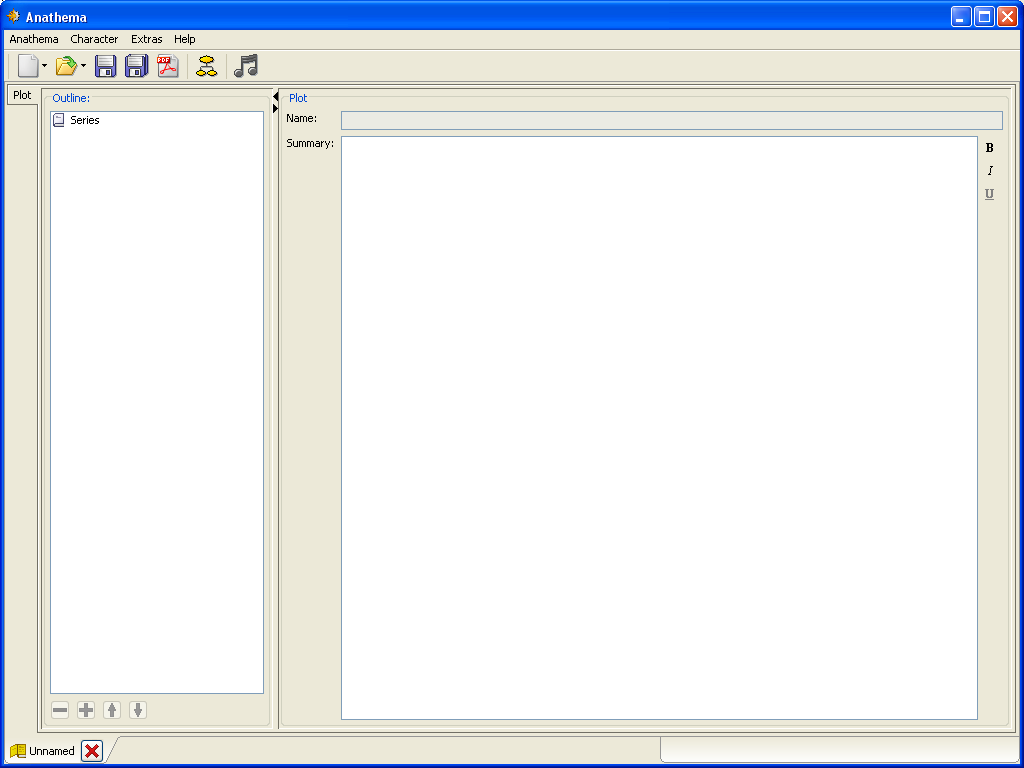
\includegraphics[width=1.00\textwidth]{images/Series.png}
	\caption{Series Screen}
	\label{fig:Series}
\end{figure}
